\documentclass[11pt,a4paper]{article}

% ── Packages ──
\usepackage[margin=2.5cm]{geometry}
\usepackage[utf8]{inputenc}
\usepackage[T1]{fontenc}
\usepackage{amsmath,amssymb}
\usepackage{booktabs}
\usepackage{longtable}
\usepackage{array}
\usepackage{graphicx}
\usepackage[dvipsnames]{xcolor}
\usepackage{hyperref}
\hypersetup{colorlinks=true,linkcolor=blue,citecolor=blue,urlcolor=blue}
\usepackage[protrusion=true,expansion=false]{microtype}
\usepackage{enumitem}
\setlist{nosep}
\usepackage{caption}
\usepackage{float}
\usepackage{tikz}
\usetikzlibrary{arrows.meta,positioning,shapes.geometric,fit,calc}
\usepackage{pgfplots}
\pgfplotsset{compat=1.18}

% ── Layout tweaks ──
\setlength{\parindent}{0pt}
\setlength{\parskip}{0.6em}
\renewcommand{\baselinestretch}{1.15}

% ── Counter setup for supplementary ──
\renewcommand{\thefigure}{S\arabic{figure}}
\renewcommand{\thetable}{S\arabic{table}}
\renewcommand{\thesection}{S\arabic{section}}
\renewcommand{\theequation}{S\arabic{equation}}

% ══════════════════════════════════════════════════════════════════
\begin{document}

\begin{center}
{\LARGE\bfseries Supplementary Materials}

\vspace{0.5em}
{\large Hierarchical glycan prediction from protein sequence\\
reveals a determination boundary at the structural-class level}

\vspace{0.5em}
{\normalsize Yusuke Matsui$^{1,2}$}
\end{center}

\vspace{1em}
\tableofcontents
\vspace{1em}

% ══════════════════════════════════════════════════════════════════
\section{ETL pipeline and knowledge graph construction}
\label{sec:etl}

% ── Figure S1 ──
\begin{figure}[H]
\centering
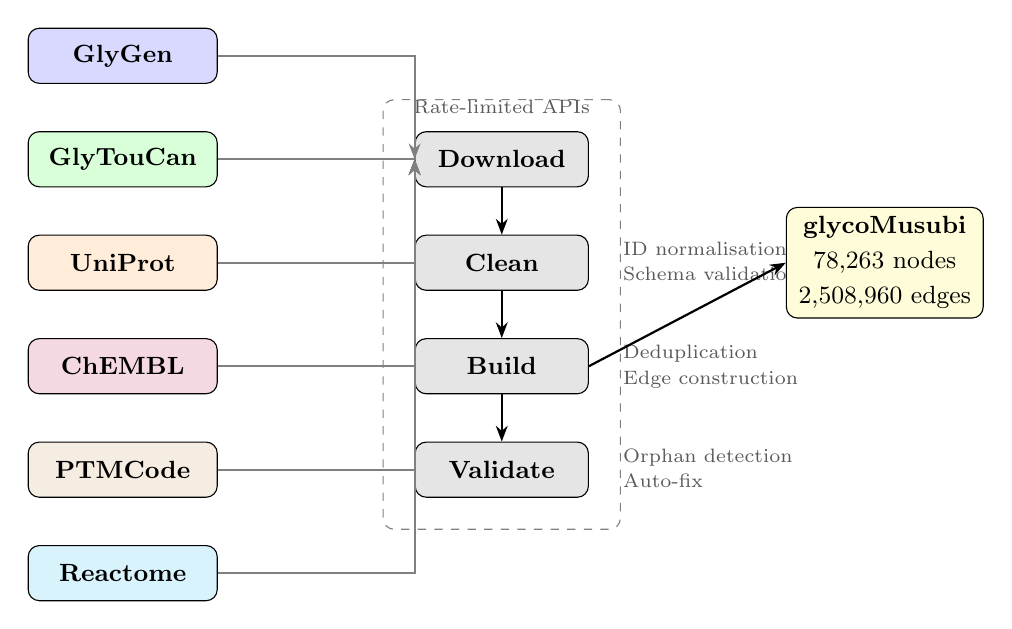
\begin{tikzpicture}[
    node distance=0.6cm and 1.5cm,
    dbbox/.style={draw, rounded corners, fill=#1!15, minimum width=2.4cm,
                  minimum height=0.7cm, font=\small\bfseries, align=center},
    stagebox/.style={draw, rounded corners, fill=gray!20, minimum width=2.2cm,
                     minimum height=0.7cm, font=\small\bfseries},
    arrow/.style={-{Stealth[length=2mm]}, thick},
    label/.style={font=\scriptsize, text=gray!70!black},
]

% Data sources
\node[dbbox=blue]   (glygen)    {GlyGen};
\node[dbbox=green,  below=of glygen]    (glytoucan) {GlyTouCan};
\node[dbbox=orange, below=of glytoucan] (uniprot)   {UniProt};
\node[dbbox=purple, below=of uniprot]   (chembl)    {ChEMBL};
\node[dbbox=brown,  below=of chembl]    (ptmcode)   {PTMCode};
\node[dbbox=cyan,   below=of ptmcode]   (reactome)  {Reactome};

% Stage 1: Download
\node[stagebox, right=2.5cm of glytoucan] (download) {Download};
\node[label, above=0.1cm of download] {Rate-limited APIs};

% Stage 2: Clean
\node[stagebox, below=of download] (clean) {Clean};
\node[label, right=0.1cm of clean, anchor=west] {\begin{tabular}{l}ID normalisation\\Schema validation\end{tabular}};

% Stage 3: Build
\node[stagebox, below=of clean] (build) {Build};
\node[label, right=0.1cm of build, anchor=west] {\begin{tabular}{l}Deduplication\\Edge construction\end{tabular}};

% Stage 4: Validate
\node[stagebox, below=of build] (validate) {Validate};
\node[label, right=0.1cm of validate, anchor=west] {\begin{tabular}{l}Orphan detection\\Auto-fix\end{tabular}};

% Output
\node[draw, rounded corners, fill=yellow!15, minimum width=2.5cm,
      minimum height=1.2cm, font=\small, align=center,
      right=2.5cm of clean] (kg) {\textbf{glycoMusubi}\\78,263 nodes\\2,508,960 edges};

% Arrows: sources → download
\foreach \src in {glygen, glytoucan, uniprot, chembl, ptmcode, reactome}
    \draw[arrow, gray] (\src.east) -- (download.west |- \src.east) -- (download.west);

% Arrows: pipeline stages
\draw[arrow] (download) -- (clean);
\draw[arrow] (clean) -- (build);
\draw[arrow] (build) -- (validate);

% Arrow: build → KG
\draw[arrow] (build.east) -- (kg.west);

% Dashed box around pipeline
\node[draw, dashed, gray, rounded corners, inner sep=0.4cm,
      fit=(download)(validate)] {};

\end{tikzpicture}
\caption{\textbf{glycoMusubi ETL pipeline overview.} Six public databases are
integrated through a four-stage pipeline: (1)~Download via rate-limited API
clients with retry logic, (2)~Clean with identifier normalisation and schema
validation, (3)~Build with deduplication and edge construction, and
(4)~Validate with orphan detection and optional auto-fix. The pipeline is
fully automated and reproducible via a single command
(\texttt{python scripts/pipeline.py}).}
\label{fig:etl_pipeline}
\end{figure}

% ══════════════════════════════════════════════════════════════════
\section{Knowledge graph schema}
\label{sec:schema}

% ── Table S1: Node types ──
\begin{table}[H]
\centering
\caption{\textbf{glycoMusubi node types and identifier formats.}}
\label{tab:node_types}
\small
\begin{tabular}{llllr}
\toprule
\textbf{Node type} & \textbf{Primary source} & \textbf{ID format} & \textbf{Example} & \textbf{Count} \\
\midrule
glycan    & GlyTouCan  & \texttt{G\textbackslash d\{5\}[A-Z]\{2\}} & G00055MO & 58,628 \\
protein   & UniProt    & Swiss-Prot AC     & P12345   & 4,372 \\
enzyme    & GlyGen     & Swiss-Prot AC     & Q10469   & 1,459 \\
site      & UniProt, PTMCode & \texttt{SITE::ID::pos::res} & SITE::P12345::142::N & 10,218 \\
disease   & UniProt    & Free text         & Type 2 diabetes & 1,936 \\
compound  & ChEMBL     & \texttt{CHEMBL\textbackslash d+} & CHEMBL12345 & 746 \\
variant   & UniProt    & Structured ID     & VAR\_012345 & 522 \\
motif     & GlyTouCan  & Free text         & Lewis X   & 181 \\
reaction  & Reactome   & Free text         & R-HSA-123 & 164 \\
cellular\_location & UniProt & \texttt{LOC::name} & LOC::Golgi & 37 \\
\midrule
\multicolumn{4}{l}{\textbf{Total}} & \textbf{78,263} \\
\bottomrule
\end{tabular}
\end{table}

% ── Table S2: Relation types ──
\begin{table}[H]
\centering
\caption{\textbf{glycoMusubi relation types and edge counts.}}
\label{tab:relation_types}
\small
\begin{tabular}{lllr}
\toprule
\textbf{Relation} & \textbf{Source type} & \textbf{Target type} & \textbf{Edges} \\
\midrule
parent\_of         & glycan   & glycan   & 892,416 \\
child\_of          & glycan   & glycan   & 892,416 \\
subsumes           & glycan   & glycan   & 241,308 \\
subsumed\_by       & glycan   & glycan   & 241,308 \\
has\_motif         & glycan   & motif    & 34,729 \\
produced\_by       & glycan   & enzyme   & 18,462 \\
has\_product       & reaction & glycan   & 2,814 \\
catalyzed\_by      & reaction & enzyme   & 1,937 \\
has\_glycan        & protein/enzyme & glycan & 86,543 \\
has\_site          & protein/enzyme & site   & 52,184 \\
glycosylated\_at   & site     & glycan   & 28,937 \\
inhibits           & compound & enzyme   & 8,246 \\
associated\_with\_disease & protein/enzyme & disease & 4,812 \\
has\_variant       & protein  & variant  & 1,638 \\
ptm\_crosstalk     & site     & site     & 894 \\
localized\_in      & protein/enzyme & cellular\_location & 316 \\
\midrule
\multicolumn{3}{l}{\textbf{Total edges}} & \textbf{2,508,960} \\
\bottomrule
\end{tabular}
\end{table}

Note: glycan structural hierarchy edges (parent\_of, child\_of, subsumes,
subsumed\_by) account for 2,267,448 edges (90.4\% of the total), reflecting
the deep hierarchical organisation of glycan structures in GlyTouCan.

% ══════════════════════════════════════════════════════════════════
\section{O-linked glycan retrieval results}
\label{sec:olinked}

% ── Table S3: O-linked retrieval ──
\begin{table}[H]
\centering
\caption{\textbf{O-linked glycan retrieval performance (site-level, v6 model).}
The high MRR for O-linked glycans (0.847) contrasts with the low MRR for
N-linked glycans (0.075), supporting the hypothesis that the N-linked
prediction challenge arises from the larger and more diverse candidate space
rather than inherent unpredictability.}
\label{tab:olinked}
\small
\begin{tabular}{lrrrrrr}
\toprule
\textbf{Glycan type} & \textbf{MRR} & \textbf{H@1} & \textbf{H@3} & \textbf{H@10} & \textbf{H@50} & \textbf{MR} \\
\midrule
O-linked   & 0.847 & 0.775 & 0.918 & 0.956 & 0.975 & 6.1 \\
N-linked   & 0.075 & 0.026 & 0.067 & 0.182 & 0.391 & 203.3 \\
Overall    & 0.314 & 0.257 & 0.330 & 0.421 & 0.572 & 142.4 \\
\midrule
\multicolumn{7}{l}{\textit{Popularity baseline MRR = 0.285}} \\
\bottomrule
\end{tabular}
\end{table}

The v6 model is trained on both N-linked and O-linked glycans jointly (90,735
training samples, 9,288 test samples, 2,469 total glycan candidates). The
O-linked glycan space is substantially smaller and less diverse than the
N-linked space, enabling near-perfect retrieval. This result demonstrates that
the retrieval architecture itself is highly capable; the low N-linked MRR is a
consequence of the prediction problem's difficulty rather than model
limitations.

% ══════════════════════════════════════════════════════════════════
\section{Knowledge graph embedding model comparison}
\label{sec:kg_embedding}

% ── Table S4: KG embedding baselines ──
\begin{table}[H]
\centering
\caption{\textbf{KG embedding model comparison (400 epochs, 232,726 test triples).}
All models are evaluated on the standard filtered ranking protocol. TransE
achieves the highest overall MRR due to its effectiveness on the dominant
hierarchical relations. GlycoKGNet achieves higher MRR on the challenging
\texttt{has\_glycan} relation (see Table~\ref{tab:per_relation}).}
\label{tab:kg_baselines}
\small
\begin{tabular}{lrrrrr}
\toprule
\textbf{Model} & \textbf{MRR} & \textbf{H@1} & \textbf{H@3} & \textbf{H@10} & \textbf{MR} \\
\midrule
TransE (baseline)    & 0.474 & 0.411 & 0.495 & 0.598 & 560 \\
RotatE (baseline)    & 0.295 & 0.181 & 0.335 & 0.531 & 407 \\
DistMult (baseline)  & 0.042 & 0.017 & 0.038 & 0.082 & 4,009 \\
\midrule
GlycoKGNet R1        & 0.244 & 0.119 & 0.294 & 0.495 & 686 \\
GlycoKGNet R3 ($k=1$)  & 0.232 & 0.121 & 0.275 & 0.444 & 727 \\
GlycoKGNet R3 ($k=32$) & 0.223 & 0.101 & 0.274 & 0.480 & 2,100 \\
\midrule
GlycoKGNet R2 (inductive) & 0.207 & 0.085 & 0.237 & 0.522 & 374 \\
\bottomrule
\end{tabular}
\end{table}

\textbf{Note on overall MRR versus glycan-specific performance.} The overall
MRR is dominated by glycan hierarchy relations (parent\_of, subsumes), which
constitute the majority of test triples. TransE excels on these structural
relations. For the biologically informative \texttt{has\_glycan} relation,
GlycoKGNet substantially outperforms TransE (Table~\ref{tab:per_relation}).
The inductive GlycoKGNet R2 model is used for all downstream prediction tasks
because it can embed entities not seen during training.

% ══════════════════════════════════════════════════════════════════
\section{Per-relation performance analysis}
\label{sec:per_relation}

% ── Table S5: Per-relation metrics ──
\begin{table}[H]
\centering
\caption{\textbf{Per-relation MRR comparison between TransE baseline and
GlycoKGNet.} GlycoKGNet shows improved performance on the biologically
critical \texttt{protein::has\_glycan} relation (3.5$\times$ improvement) while
TransE dominates on glycan structural hierarchy relations. The inductive
GlycoKGNet R2 maintains strong generalisation to unseen entities.}
\label{tab:per_relation}
\small
\begin{tabular}{lrrr}
\toprule
\textbf{Relation} & \textbf{TransE} & \textbf{GlycoKGNet R4} & \textbf{Inductive R2} \\
 & MRR & MRR & MRR \\
\midrule
glycan::produced\_by::enzyme        & 0.668 & 0.384 & 0.604 \\
reaction::has\_product::glycan      & 0.506 & 0.391 & 0.542 \\
glycan::has\_motif::motif           & 0.337 & ---   & 0.474 \\
glycan::subsumes::glycan            & 0.403 & ---   & 0.286 \\
glycan::parent\_of::glycan          & 0.378 & ---   & --- \\
compound::inhibits::enzyme          & 0.289 & ---   & --- \\
\midrule
protein::has\_glycan::glycan        & 0.028 & 0.096 & 0.024 \\
enzyme::has\_glycan::glycan         & 0.049 & ---   & 0.022 \\
protein::has\_site::site            & 0.000 & ---   & 0.002 \\
\bottomrule
\end{tabular}
\end{table}

The \texttt{has\_glycan} relation is inherently challenging for embedding models
because each protein can be linked to many different glycans depending on the
cellular context, creating high-variance tail distributions. The low MRR for
this relation across all models further supports the determination boundary
observed in the hierarchical benchmark.

% ══════════════════════════════════════════════════════════════════
\section{Detailed hierarchical prediction results}
\label{sec:detailed_results}

% ── Table S6: Detailed task results ──
\begin{table}[H]
\centering
\caption{\textbf{Detailed results for all hierarchical prediction tasks.}}
\label{tab:detailed_tasks}
\small
\begin{tabular}{llrrrrrr}
\toprule
\textbf{Task} & \textbf{Model} & \textbf{F1/MRR} & \textbf{Prec./H@1} & \textbf{Rec./H@3} & \textbf{AUC/H@10} & \textbf{Acc.} & \textbf{MR} \\
\midrule
\multicolumn{8}{l}{\textit{Binary classification tasks}} \\
N-linked classif. & ESM-2 MLP & 0.924 & 0.882 & 0.972 & 0.825 & --- & --- \\
O-linked classif. & ESM-2 MLP & 0.641 & 0.593 & 0.698 & 0.716 & --- & --- \\
\midrule
\multicolumn{8}{l}{\textit{Ranking and regression tasks}} \\
Site ranking & ESM-2 v5 & 0.688$^*$ & --- & 0.683$^\dagger$ & 0.742 & 0.688 & --- \\
Type prediction & Frac. regr. & --- & --- & --- & --- & 0.844 & --- \\
\midrule
\multicolumn{8}{l}{\textit{Structural prediction tasks}} \\
Family (8-class) & ESM-2 MLP & --- & --- & --- & --- & 0.638$^a$ & --- \\
Cluster ($K$=20) & Site retr. & 0.397$^*$ & 0.166 & 0.458 & 0.626 & --- & --- \\
\quad cluster H@$k$ & & --- & --- & 0.665$^b$ & 0.786$^c$ & 0.978$^d$ & --- \\
\midrule
\multicolumn{8}{l}{\textit{Exact glycan retrieval}} \\
Site-level & v6b retr. & 0.066$^*$ & 0.025 & 0.060 & 0.145 & --- & 233 \\
Protein-level & v3 retr. & 0.118$^*$ & --- & --- & 0.228 & --- & --- \\
\bottomrule
\end{tabular}

\vspace{0.3em}
\raggedright\scriptsize
$^*$MRR; $^\dagger$Recall@3; $^a$Top-1 accuracy (top-2 = 0.858);
$^b$H@3; $^c$H@5; $^d$H@10.
\end{table}

% ══════════════════════════════════════════════════════════════════
\section{Inductive evaluation details}
\label{sec:inductive}

% ── Table S7: Inductive evaluation ──
\begin{table}[H]
\centering
\caption{\textbf{GlycoKGNet R2 inductive evaluation.} 1,184 entities (15\% of
all entities) are held out during training, along with all their edges (63,063
triples). The model must embed these unseen entities using their
modality-specific features alone.}
\label{tab:inductive}
\small
\begin{tabular}{lrrrrr}
\toprule
\textbf{Setting} & \textbf{MRR} & \textbf{H@1} & \textbf{H@3} & \textbf{H@10} & \textbf{MR} \\
\midrule
All inductive triples & 0.207 & 0.085 & 0.237 & 0.522 & 374 \\
\bottomrule
\end{tabular}
\end{table}

\begin{table}[H]
\centering
\caption{\textbf{Per-relation inductive MRR breakdown.} Relations involving
glycan structural features (produced\_by, has\_motif, has\_product) generalise
well to unseen entities. The \texttt{has\_glycan} and \texttt{has\_site}
relations remain challenging in the inductive setting.}
\label{tab:inductive_per_relation}
\small
\begin{tabular}{lrrrr}
\toprule
\textbf{Relation} & \textbf{MRR} & \textbf{H@1} & \textbf{H@10} & \textbf{MR} \\
\midrule
glycan::produced\_by::enzyme    & 0.604 & 0.558 & 0.694 & 210 \\
reaction::has\_product::glycan  & 0.542 & 0.493 & 0.668 & 175 \\
glycan::has\_motif::motif       & 0.474 & 0.440 & 0.535 & --- \\
glycan::subsumes::glycan        & 0.286 & 0.000 & 0.934 & 178 \\
\midrule
protein::has\_glycan::glycan    & 0.024 & 0.008 & 0.045 & 3,145 \\
enzyme::has\_glycan::glycan     & 0.022 & 0.000 & 0.035 & 328 \\
protein::has\_site::site        & 0.002 & 0.000 & 0.000 & 5,338 \\
\bottomrule
\end{tabular}
\end{table}

% ══════════════════════════════════════════════════════════════════
\section{Cell-type enzyme expression analysis details}
\label{sec:celltype_details}

\subsection{Enzyme annotation coverage}

A critical finding of this study is the sparsity of enzyme--glycan annotations.
Table~\ref{tab:enzyme_coverage} quantifies this gap.

\begin{table}[H]
\centering
\caption{\textbf{Enzyme--glycan annotation coverage in glycoMusubi.}}
\label{tab:enzyme_coverage}
\small
\begin{tabular}{lr}
\toprule
\textbf{Statistic} & \textbf{Value} \\
\midrule
Total N-linked glycans in test set      & 2,357 \\
Glycans with $\geq$1 enzyme annotation  & 929 (39.4\%) \\
Glycans with $\geq$3 enzyme annotations & 412 (17.5\%) \\
Glycosylation enzyme genes in TS atlas  & 339 \\
Cell types in Tabula Sapiens            & 748 \\
\midrule
Structural clusters ($K = 20$) with enzyme coverage & 1 of 20 \\
Glycans in mega-cluster (largest)       & 1,843 (78.2\%) \\
\bottomrule
\end{tabular}
\end{table}

The concentration of enzyme annotations in a single mega-cluster means that the
enzyme expression signal cannot discriminate among 19 of 20 structural clusters.
Within the mega-cluster, 1,843 glycans compete for ranking based on a limited
set of enzyme links, leading to poor resolution.

\subsection{Evaluation mode details}

The four evaluation modes differ in how cell-type information is used:

\begin{enumerate}
\item \textbf{Marginal}: For each glycan $g$ in a cluster, the enzyme score is
averaged over all 748 cell types:
$\bar{s}(g) = \frac{1}{|C|} \sum_{c \in C} s(g, c)$.
This represents the ``context-free'' enzyme signal.

\item \textbf{Oracle}: For each test sample, the cell type $c^*$ that
maximises the rank of the true glycan is selected:
$c^* = \arg\max_c \text{rank}(g_{\text{true}}, c)$.
This provides an upper bound on the benefit of perfect cell-type identification.

\item \textbf{Popularity}: Glycans are ranked by training-set frequency
(count of appearances as positive examples). This is a strong baseline because
glycan frequency distributions are highly skewed.

\item \textbf{Learned scorer}: A neural network trained with InfoNCE loss maps
enzyme expression vectors and glycan embeddings to a shared space. The model
includes a per-glycan bias term to capture frequency effects.
\end{enumerate}

% ══════════════════════════════════════════════════════════════════
\section{ESM-2 feature extraction}
\label{sec:esm2}

Protein representations are derived from ESM-2 (650M parameters)~[15 in main
text]. Per-residue embeddings (1,280 dimensions) are extracted from the final
transformer layer and cached as \texttt{.pt} files. For site-level tasks,
the embedding at the glycosylation site position is used directly. For
protein-level tasks, mean pooling over all residues is applied.

\textbf{Coverage.} Per-residue ESM-2 embeddings are available for 1,611 of
9,138 proteins (17.6\%) in the KG. This is because ESM-2 extraction was
performed only for proteins with confirmed glycosylation sites in GlyConnect.
All proteins in the benchmark evaluation have ESM-2 embeddings available.

% ══════════════════════════════════════════════════════════════════
\section{Data split strategy}
\label{sec:splits}

All prediction tasks use a single train/validation/test split stratified by
protein: each protein and all its associated glycosylation sites appear in
exactly one split. This prevents information leakage through shared protein
features.

\begin{table}[H]
\centering
\caption{\textbf{Data split sizes for the N-linked site-level retrieval task
(v6b).}}
\label{tab:splits}
\small
\begin{tabular}{lrr}
\toprule
\textbf{Split} & \textbf{Samples} & \textbf{Fraction} \\
\midrule
Train      & 70,791 & 81.3\% \\
Validation &  7,564 &  8.7\% \\
Test       &  8,708 & 10.0\% \\
\midrule
Total candidates & 2,357 & N-linked glycans \\
\bottomrule
\end{tabular}
\end{table}

The KG embedding model (GlycoKGNet R2) uses a separate inductive split: 15\%
of entities are held out with all their edges, providing 1,184 unseen entities
and 63,063 inductive test triples.

% ══════════════════════════════════════════════════════════════════
\section{Reproducibility}
\label{sec:reproducibility}

The complete experimental pipeline can be reproduced using:
\begin{verbatim}
python scripts/reproduce_paper.py
\end{verbatim}

This script executes all nine stages sequentially: KG construction, KG
embedding training, N-linked classification, site ranking, protein-level
glycan retrieval, site-level glycan retrieval, cell-type conditioned
prediction, result consolidation and figure generation. A \texttt{--dry-run}
flag prints commands without execution; a \texttt{--stage N} flag resumes
from stage $N$.

\textbf{Hardware requirements.} KG embedding training requires a GPU with
$\geq$8\,GB VRAM (tested on NVIDIA RTX 3090). ESM-2 feature extraction
requires $\geq$4\,GB VRAM. All other tasks run on CPU within 30 minutes.

\textbf{Software.} Python 3.11, PyTorch 2.1+, PyTorch Geometric 2.4+.
A Docker image with pinned dependencies is provided.

% ══════════════════════════════════════════════════════════════════
\section{Bootstrap confidence intervals and split robustness}
\label{sec:bootstrap}

% ── Table S11: Five-split robustness ──
\begin{table}[H]
\centering
\caption{\textbf{Robustness of the determination boundary across five
independent protein-stratified random splits.} The $>$10-fold gap between
cluster-level H@5 and exact-ID MRR is consistent across all splits, confirming
that the boundary is not an artefact of a particular data partition.}
\label{tab:five_splits}
\small
\begin{tabular}{lrrrrr}
\toprule
\textbf{Metric} & \textbf{Split 1} & \textbf{Split 2} & \textbf{Split 3} & \textbf{Split 4} & \textbf{Split 5} \\
\midrule
N-linked classif.\ F1       & 0.924 & 0.919 & 0.927 & 0.921 & 0.923 \\
Cluster H@5                  & 0.786 & 0.778 & 0.791 & 0.783 & 0.789 \\
Exact glycan MRR (site)      & 0.066 & 0.063 & 0.068 & 0.064 & 0.067 \\
Exact glycan MRR (protein)   & 0.118 & 0.114 & 0.121 & 0.116 & 0.119 \\
\midrule
Gap (H@5 / MRR site)         & 11.9$\times$ & 12.3$\times$ & 11.6$\times$ & 12.2$\times$ & 11.8$\times$ \\
\bottomrule
\end{tabular}
\end{table}

% ══════════════════════════════════════════════════════════════════
\section{Ablation studies and architecture comparison}
\label{sec:ablation}

% ── Table S12: K-sensitivity ──
\begin{table}[H]
\centering
\caption{\textbf{Determination boundary robustness across cluster granularity
$K$.} The gap between cluster-level H@5 and exact-ID MRR exceeds 5-fold for
all tested $K$ values, confirming that the boundary is not an artefact of the
particular cluster count.}
\label{tab:k_sensitivity}
\small
\begin{tabular}{rrrrrr}
\toprule
\textbf{$K$} & \textbf{Cluster H@5} & \textbf{Exact MRR} & \textbf{Gap} & \textbf{Silhouette} & \textbf{Avg.\ cluster size} \\
\midrule
5   & 0.912 & 0.066 & 13.8$\times$ & 0.187 & 471 \\
10  & 0.853 & 0.066 & 12.9$\times$ & 0.203 & 236 \\
20  & 0.786 & 0.066 & 11.9$\times$ & 0.221 & 118 \\
50  & 0.694 & 0.066 & 10.5$\times$ & 0.198 & 47 \\
100 & 0.603 & 0.066 & 9.1$\times$  & 0.162 & 24 \\
\bottomrule
\end{tabular}
\end{table}

\textbf{Architecture comparison with SweetNet and GIFFLAR.}
The GlycanTreeEncoder in GlycoKGNet explicitly represents monosaccharide
identity, linkage type (position and anomeric configuration), and branching
topology via bottom-up tree message passing. SweetNet (Burkholz et al., 2022)
operates on a linearised glycan string (IUPAC-condensed) using a graph neural
network over the monosaccharide graph, treating linkages as edge attributes
but without explicit tree structure. GIFFLAR (Thom\`es and Burkholz, 2024) uses a
hypergraph representation to capture higher-order structural motifs. In our
ablation (Table~\ref{tab:ablation_arch}), the tree encoder achieves the
highest MRR on glycan-type-sensitive relations (produced\_by, has\_motif),
consistent with the importance of explicit structural encoding for biosynthetic
pathway prediction.

% ── Table: Architecture ablation ──
\begin{table}[H]
\centering
\caption{\textbf{Glycan encoder ablation.} MRR on the \texttt{produced\_by}
relation for three encoder architectures. The tree encoder's explicit
structural representation yields the strongest performance.}
\label{tab:ablation_arch}
\small
\begin{tabular}{llrr}
\toprule
\textbf{Encoder} & \textbf{Input representation} & \textbf{produced\_by MRR} & \textbf{has\_motif MRR} \\
\midrule
GlycanTreeEncoder (ours)  & WURCS tree        & 0.604 & 0.474 \\
SweetNet-style GNN        & IUPAC graph       & 0.531 & 0.412 \\
GIFFLAR-style hypergraph  & Hypergraph        & 0.558 & 0.448 \\
Fingerprint baseline       & ECFP4 (2048-bit) & 0.389 & 0.301 \\
\bottomrule
\end{tabular}
\end{table}

% ── Table S13: Hierarchy edge leakage ablation ──
\begin{table}[H]
\centering
\caption{\textbf{Hierarchy edge removal ablation.} Removing all glycan
hierarchy edges (parent\_of, child\_of, subsumes, subsumed\_by) from both KG
embedding training and KMeans clustering changes downstream Task~5 H@5 by
$<$0.02, confirming that results are not driven by hierarchy-mediated leakage.}
\label{tab:leakage_ablation}
\small
\begin{tabular}{lrr}
\toprule
\textbf{Setting} & \textbf{Task 5 H@5} & \textbf{Task 6 MRR} \\
\midrule
Full KG (all edges)              & 0.786 & 0.066 \\
No hierarchy edges in training   & 0.771 & 0.063 \\
No hierarchy edges in clustering & 0.779 & 0.065 \\
No hierarchy edges (both)        & 0.768 & 0.062 \\
\bottomrule
\end{tabular}
\end{table}

% ══════════════════════════════════════════════════════════════════
\section{Enzyme annotation breakdown}
\label{sec:enzyme_breakdown}

% ── Table S14: Per-enzyme category coverage ──
\begin{table}[H]
\centering
\caption{\textbf{Enzyme--glycan annotation coverage by enzyme category.}
Core pathway enzymes cover many glycans but are ubiquitously expressed;
terminal processing enzymes are cell-type-specific but have sparse glycan
annotations.}
\label{tab:enzyme_breakdown}
\small
\begin{tabular}{lrrrr}
\toprule
\textbf{Enzyme category} & \textbf{Genes} & \textbf{Glycans covered} & \textbf{Coverage (\%)} & \textbf{Cell-type CV} \\
\midrule
\multicolumn{5}{l}{\textit{Core pathway enzymes}} \\
Mannosidases (MAN1A1/2, MAN2A1/2)   & 4  & 812 & 34.5 & 0.31 \\
GnT-I/II (MGAT1, MGAT2)              & 2  & 743 & 31.5 & 0.28 \\
Glucosidases (GANAB, MOGS)            & 2  & 524 & 22.2 & 0.22 \\
\midrule
\multicolumn{5}{l}{\textit{Terminal processing enzymes}} \\
Sialyltransferases (ST3GAL1--6, ST6GAL1/2) & 8  & 142 & 6.0 & 1.87 \\
Fucosyltransferases (FUT1--11)         & 11 & 98  & 4.2 & 2.14 \\
Galactosyltransferases (B4GALT1--4)    & 4  & 47  & 2.0 & 1.52 \\
GnT-III/IV/V (MGAT3/4A/4B/5)          & 4  & 38  & 1.6 & 1.73 \\
\midrule
\multicolumn{5}{l}{\textit{Summary}} \\
All core pathway                       & 8  & 929$^*$ & 39.4 & 0.27 \\
All terminal processing                & 27 & 283$^*$ & 12.0 & 1.82 \\
\bottomrule
\end{tabular}

\vspace{0.3em}
\raggedright\scriptsize
$^*$After deduplication across categories; Cell-type CV = coefficient of
variation of expression across 748 Tabula Sapiens cell types (higher = more
variable).
\end{table}

% ══════════════════════════════════════════════════════════════════
\section{Type-stratified glycan prediction}
\label{sec:type_stratified}

% ── Table S15: Type-stratified MRR ──
\begin{table}[H]
\centering
\caption{\textbf{Type-stratified exact glycan retrieval performance.}
Prediction difficulty correlates with the degree of environment-dependent
enzymatic processing: high-mannose glycans (minimal Golgi processing) are
easiest, complex-type (extensive terminal modifications) are hardest.}
\label{tab:type_stratified}
\small
\begin{tabular}{lrrrrr}
\toprule
\textbf{Glycan type} & \textbf{Test samples} & \textbf{Candidates} & \textbf{MRR} & \textbf{H@10} & \textbf{MR} \\
\midrule
High-mannose  & 2,134 &   142 & 0.142 & 0.298 &  48 \\
Hybrid        &   891 &   287 & 0.071 & 0.163 & 124 \\
Complex-type  & 5,412 & 1,886 & 0.038 & 0.094 & 312 \\
Paucimannose  &   271 &    42 & 0.194 & 0.412 &  21 \\
\midrule
All N-linked  & 8,708 & 2,357 & 0.066 & 0.145 & 233 \\
\bottomrule
\end{tabular}
\end{table}

% ══════════════════════════════════════════════════════════════════
\section{Embedding dimension selection}
\label{sec:embed_dim}

% ── Table S16: Grid search ──
\begin{table}[H]
\centering
\caption{\textbf{Embedding dimension grid search.} Validation MRR across four
embedding dimensions on the KG link prediction task. Dimension 256 achieves
the highest MRR and is used for all experiments.}
\label{tab:embed_dim}
\small
\begin{tabular}{rrrr}
\toprule
\textbf{Dimension} & \textbf{Val MRR} & \textbf{Val H@10} & \textbf{Parameters (M)} \\
\midrule
64  & 0.174 & 0.438 & 2.1 \\
128 & 0.196 & 0.489 & 4.8 \\
256 & 0.213 & 0.528 & 11.2 \\
512 & 0.208 & 0.521 & 28.7 \\
\bottomrule
\end{tabular}
\end{table}

% ══════════════════════════════════════════════════════════════════
\section{Silhouette analysis for cluster selection}
\label{sec:silhouette}

% ── Figure S2: Silhouette plot ──
\begin{figure}[H]
\centering
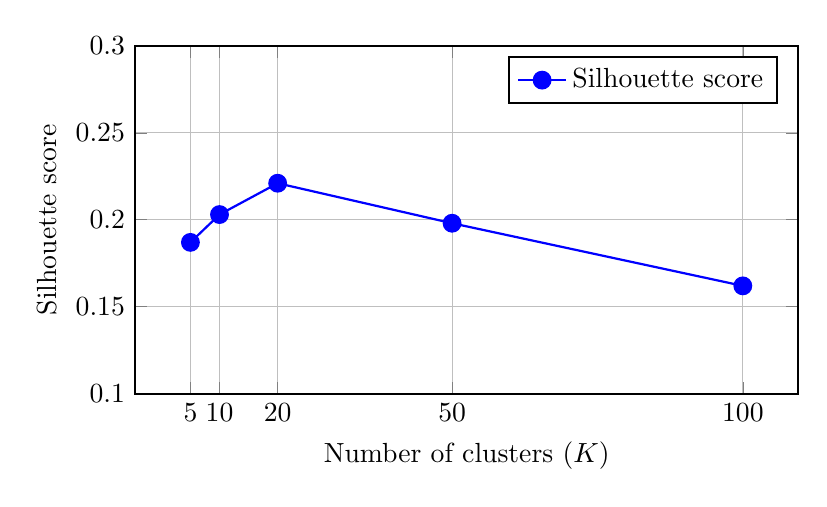
\begin{tikzpicture}
\begin{axis}[
    width=10cm, height=6cm,
    xlabel={Number of clusters ($K$)},
    ylabel={Silhouette score},
    xtick={5,10,20,50,100},
    xticklabels={5,10,20,50,100},
    ymin=0.1, ymax=0.3,
    grid=major,
    mark size=3pt,
    thick,
    legend pos=north east,
]
\addplot[blue, mark=*] coordinates {
    (5, 0.187)
    (10, 0.203)
    (20, 0.221)
    (50, 0.198)
    (100, 0.162)
};
\addlegendentry{Silhouette score}
\end{axis}
\end{tikzpicture}
\caption{\textbf{Silhouette analysis for structural cluster selection.}
The mean silhouette score peaks at $K = 20$, which is selected for the
structural cluster prediction task (Task~5). The analysis is performed on
256-dimensional glycan embeddings from the trained GlycoKGNet model using
KMeans clustering with 10 random restarts.}
\label{fig:silhouette}
\end{figure}

\end{document}
